\section{Derivatives of VVFs}
\noindent
Just like functions from Calc I and II, we can differentiate VVFs.
In fact, the limit definitions of the derivative are nearly identical.
Let $\vec{r}(t) = \langle x(t), y(t), z(t) \rangle$.
\begin{align*}
	\vec{r^\prime}(t) &= \lim_{h\to 0}{\frac{\vec{r}(t+h)-\vec{r}(t)}{h}} \\
	&= \lim_{h\to 0}{\bigg\langle \frac{x(t+h)-x(t)}{h}, \frac{y(t+h)-y(t)}{h}, \frac{z(t+h)-z(t)}{h} \bigg\rangle}.
\end{align*}
The limit distributes inside the vector, so
\begin{equation*}
	\vec{r^\prime}(t) = \langle x^{\prime}(t), y^{\prime}(t), z^{\prime}(t) \rangle.
\end{equation*}

\noindent
Like a position function from Calc I and II, the derivative of a VVF representing position gives a VVF representing velocity, and the 2nd derivative gives a VVF representing acceleration.
The magnitude of the velocity VVF, the speed, is commonly notated $v(t)$.\\

\noindent
There are 5 important properties of the derivatives of VVFs.
These properties are similar to single-variable derivatives.
Let $\vec{r}(t)$ and $\vec{s}(t)$ be VVFs, $a(t)$ be a scalar function, and $c$ be a scalar.
\begin{enumerate}[label=]
	\item \textbf{Linearity}
	\begin{equation*}
		\frac{\mathrm{d}}{\mathrm{d}t}c\vec{r}(t) = c\vec{r^\prime}(t)
	\end{equation*}
	\item \textbf{Product Rule for Scalar Functions}
	\begin{equation*}
		\frac{\mathrm{d}}{\mathrm{d}t}a(t)\vec{r}(t) = a(t)\vec{r^\prime}(t) + \vec{r}(t)a^{\prime}(t)
	\end{equation*}
	\item \textbf{Dot Product Rul}e
	\begin{equation*}
		\frac{\mathrm{d}}{\mathrm{d}t}\vec{s}(t)\cdot\vec{r}(t) = \vec{s}(t)\cdot\vec{r^\prime}(t) + \vec{r}(t)\vec{s^\prime}(t)
	\end{equation*}
	\item \textbf{Cross Product Rule}
	\begin{equation*}
		\frac{\mathrm{d}}{\mathrm{d}t}\vec{s}(t)\times\vec{r}(t) = \vec{s}(t)\times\vec{r^\prime}(t) + \vec{s^\prime}(t)\times\vec{r}(t)
	\end{equation*}
	\item \textbf{Chain Rule}
	\begin{equation*}
		\frac{\mathrm{d}}{\mathrm{d}t}\vec{r}(a(t)) = \vec{r^\prime}(a(t))a^{\prime}(t)
	\end{equation*}
\end{enumerate}
A quotient rule doesn't make sense because we don't have an operation for dividing two vectors by each other.\\

\noindent
Just like in single variable calculus, we can use the derivative of VVFs to find tangent lines to the curve.
Similar to how $f^{\prime}(a)$ represents the slope of $f$ at $a$, $\vec{r^\prime}(a)$ represents the direction of the tangent line at $a$.
Remembering the VVF form of a line, the tangent line to $\vec{r}$ at $t$ is 
\begin{equation*}
	\vec{l}(t)=\vec{r}(t)+t\vec{r^\prime}(t).
\end{equation*}
In fact, tangent lines appear so often, that we have a special unit vector representing the direction of the tangent line.
\begin{equation*}
	\hat{T}(t) = \frac{\vec{r^\prime}(t)}{\norm{\vec{r^\prime}(t)}}.
\end{equation*}
You can remember $\hat{T}$ as the ``tangent'' vector.

\begin{figure}[H]
	\centering
	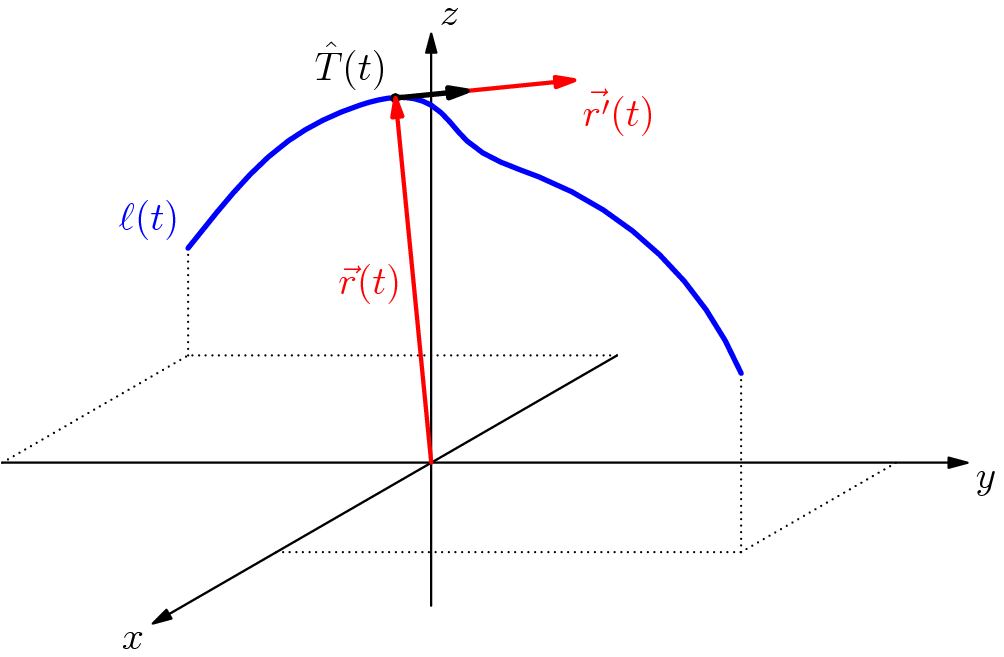
\includegraphics[scale=0.33]{Images/vectorValuedFunctions/TangentVector}
	\caption{$\hat{T}$ is $\vec{r^\prime}$ normalized.}
\end{figure}